\subsection{Calculus}

We assume that incoming graduate students have completed coursework in calculus including the basic calculation of derivatives, antiderivatives, definite integrals, series/sequences, and multivariate calculus. Below are outlined some more advanced calculus concepts that have specific physical relevance to concepts covered in the MSE core.

Any college-level calculus text is suitable for supplemental study. The sections below on Total Differentials (Sec. \ref{subsec:totdiff}) and Exact/Inexact Differentials (Sec. \ref{subsec:eidiff}) were adapted from the course materials of Richard Fitzpatrick at UT-Austin (available \href{http://farside.ph.utexas.edu/teaching/sm1/Thermal.pdf}{here}).
	
\subsubsection{Total Differentials: \hfill(Release 11/2016)} \label{subsec:totdiff}

\textit{\textbf{Encountered in: MAT\texttt{\_}SCI 401}} 
	
When there exists an explicit function of several variables such as $f = f(x,y,t)$, which has $f$ has a \emph{total} differential of form:
%
\begin{align}
	\Diff{}{f} = \Big(\Partial{}{f}{t}\Big)_{x,y}\Diff{}{t} + \Big(\Partial{}{f}{x}\Big)_{t,y} \Diff{}{x} + \Big(\Partial{}{f}{y}\Big)_{t,x} \Diff{}{y}
\end{align}
%
Here, we do not assume that $f$ is constant with respect any of the arguments $(x\text{,}\, y\text{, or } t)$. This equation defines the differential change in the function $\Diff{}{f}$ and accounts for all interdependencies between $x$, $y$, and $t$. In general, the total differential can be defined as:
%
\begin{align} \label{eq:TotDiff}
	\Diff{}{f} = \sum\limits_{i=1}^n \Big(\Partial{}{f}{x_i}\Big)_{x_{j\neq i}}\Diff{}{x_i}
\end{align}
%
The total differential is important when working with thermodynamic systems which is described by thermodynamic parameters (e.g. $P$, $T$, $V$) which are not necessary independent. For example, the internal energy $U$ for some homogeneous system can be defined in terms of entropy $S$ and volume $V$; $U = U(S,V)$. According to Eq. \ref{eq:TotDiff}, the infinitesimal change in internal entropy is therefore:
%
 \begin{align}
	\Diff{}{U} = \Big(\Partial{}{U}{S}\Big)_{V}\Diff{}{S} + \Big(\Partial{}{U}{V}\Big)_{S} \Diff{}{V}
\end{align}
%
	\subsubsection{Exact and Inexact Differentials \hfill(Release 11/2016)} \label{subsec:eidiff}
	
	\textit{\textbf{Encountered in: MAT\texttt{\_}SCI 401}} 
	
Suppose we are assessing the infinitesimal change of some value: $\Diff{}{f}$, in which $\Diff{}{f}$ is a linear differential of the form:
%
\begin{align}
	\Diff{}{f} = \sum\limits_{i=1}^m M_i(x_1,x_2,...x_m)\Diff{}{x_i}.
\end{align}
%	
In thermodynamics we are often concerned with linear differentials of two independent variables such that 
%
\begin{align} \label{eq:LinearDiff}
	\Diff{}{f} = M(x,y) \Diff{}{x} + N(x,y) \Diff{}{y}.
\end{align}
%
An exact differential is one in which $\int{\Diff{}{z}}$ is path-independent. It can be shown (e.g. \href{http://mathworld.wolfram.com/ExactDifferential.html}{Wolfram Exact Differential}) that this means:
%
\begin{align} \label{eq:ExactDiff}
	\Diff{}{f} = \Big(\Partial{}{f}{x}\Big)_{y} \Diff{}{x} + \Big(\Partial{}{f}{y}\Big)_{x} \Diff{}{y}.
\end{align}
%
Which means that
%
\begin{align} \label{eq:ExactDiff2}
 \Big(\Partial{}{M}{y}\Big)_{x} = \Big(\Partial{}{N}{x}\Big)_{y}. %Wolfram proof.
\end{align}
%
An inexact differential is one in which the equality defined in Eq. \ref{eq:ExactDiff} (and therefore Eq. \ref{eq:ExactDiff2}) is not necessary true. An inexact differential is typically denoted using \textit{bar} notation to define the infinitesimal value:
%
\begin{align}
	\text{\dj} f = \Big(\Partial{}{f}{x}\Big)_{y} \Diff{}{x} + \Big(\Partial{}{f}{y}\Big)_{x} \Diff{}{y}.
\end{align}
%
Two physical examples make this more clear:  %This example is adapted from Safkan on StackExchange. I like it.

\begin{displayquote}
%This example is adapted from Safkan on StackExchange. I like it.
	\textbf{Example 1:} Imagine you are speaking with a classmate who recently traveled from from Chicago to Minneapolis. You know he is now in Minneapolis. Is it possible for you to know how much money he spent gas ($G$)? No, you can't. $G$ is dependent on \emph{how} your friend traveled to Minneapolis: his gas mileage, the cost of gas, and, of course, the route he took. $G$ cannot be known without understanding the details of the path, and is therefore not path independent. The differenitial of $G$ is therefore \emph{inexact}: \text{\dj}$G$.
	
	Now, what do we know about your friend's distance, $D$, to Chicago? This value does not dependent on how he traveled, the only information you need to know is his location, now, in Minneapolis. His distance to Chicago, therefore is a state variable and $\Diff{}{D}$ is an \emph{exact} differential. %Might be better to describe this as a gravitational potential energy, even.
\end{displayquote}

\begin{displayquote}%This example is adapted from Safkan on StackExchange. I like it.
	\textbf{Example 2:} Let's reconsider a situation like that of Example 1 this within the purview of thermodynamics. Consider the internal energy  $U$ of a closed system. To achieve an infinitesimal change in energy $\Diff{}{U}$, we provided a bit of work $\text{\dj}W$ or heat $\text{\dj}Q$:  $\Diff{}{U} = \text{\dj}W + \text{\dj}Q$ \footnote{sometimes, an inexact differential will be denoted as $\delta f$}. The work performed and heat exchanged on the system is path-dependent --- the total work done depends on \emph{how} the work was performed or heat exchanged, and so $\text{\dj}W$ and $\text{\dj}Q$ are inexact.
\end{displayquote}
	
It is sometimes useful to ask yourself about the nature of a variable to ascertain whether the differential is exact or inexact. That is, it makes sense to ask yourself: ``what is the energy of the system?'' or ``what is the pressure of the system''? This often helps in the identification of a state variable. However, it does not make sense to ask yourself ``what is the work of the system'' or ``what is the heat'' of the system --- these values depend on the process. Instead, you have to ask yourself: ``what is the work done on the system along this path?'' or ``what is the heat exchanged during this process?''.

Finally, there are different properties we encounter during the evaluation exact differential (such as the linear differential in Eq. \ref{eq:LinearDiff}), and inexact differentials (written as $\text{\dj}f = M'(x,y) \Diff{}{x} + N'(x,y) \Diff{}{y}$). The integral of an exact differential over a closed path is necessary zero:
%
\begin{align}
	\oint\Diff{}{f} \equiv 0,
\end{align}
%
while the integral of an inexact differential over a closed path is not \emph{necessarily} zero:
%
\begin{align}
	\oint\text{\dj}f\underset{n}{\neq} 0.
\end{align}
%
where $\Big(\underset{n}{\neq}\Big)$ symbolizes ``not necessarily equal to''. Indeed, when evaluating the inexact differential, it is important to consider the path. For example, the work performed a system going from a macrostate $s_i$ to a macrostate $s_2$ is defined by path $L_{1}$, then the total work performed is defined:
%
\begin{align}
	W_{L_{1}} =  \int\limits_{L_{1}} \text{\dj}W
\end{align}
%
If we took a different path, $L_{2}$, the total work performed by be different and
%
\begin{align}
	W_{L_{1}} \underset{n}{\neq}  W_{L_{2}}
\end{align}
%
A good illustration of a line integral over a scalar field is shown in the multimedia Fig. \ref{fig:LineIntegral}. It is clear that, depending on the path, the evaluated integral will have different values.

\begin{figure}%Converted GIF to flv. Some loss in quality. Can embed in YouTube if better.
	\centering
	\includemedia[
		width=0.4\linewidth,
		height=0.3\linewidth,
		activate=pageopen,
		addresource=./Figures/LineIntegralScalarField.flv,
		flashvars={source=./Figures/LineIntegralScalarField.flv}
	]{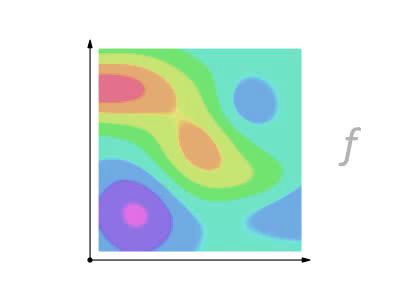
\includegraphics{./Figures/LineIntegralScalarField.png}}{VPlayer9.swf}
	\caption{An illustration of a line integral along a path in a scalar field, by Lucas V. Barbosa (own work) [Public Domain], via Wikipedia Commons. When using Adobe Pro, allow all multimedia. Click on the figure to run.}%\ref{https://en.wikipedia.org/wiki/Line\_integral\#/media/File:Line\_integral\_of\_scalar\_field.gif}{Wikipedia Commons}
	\label{fig:LineIntegral}%
\end{figure}

	\subsubsection{Vector Calculus \hfill(Release TBD)}
	
	\textit{\textbf{Encountered in: MAT\texttt{\_}SCI 406, 408}} 